\documentclass[aps,pra,reprint,amsmath,amssymb]{revtex4-1}

\usepackage{subfigure,dcolumn}
\usepackage[T2A,T1]{fontenc}
\usepackage[english]{babel}

\usepackage{braket}
\usepackage{graphicx}
\usepackage[colorinlistoftodos]{todonotes}
\usepackage[utf8]{inputenc}

% The following package will be used to typeset the LaTeX codes and is not a necessity to this template
\usepackage{listings}
\lstloadlanguages{[LaTeX]TeX}
\lstset{language=[LaTeX]TeX,keywordstyle=\color{red},showspaces=true,breaklines=true,breakatwhitespace=true,basicstyle=\small\tt,commentstyle=\color{white},frame=single,framerule=0pt,backgroundcolor=\color{yellow}}


\begin{document}


\title{Causality and the N-photon Scattering matrix in waveguide QED}

\author{...}
\affiliation{...}
\email[Corresponding author, ]{The name, complete address, telephone number, and e-mail address of the author to whom correspondence and proofs should be sent.}


\begin{abstract}
The scattering matrix $S$ is one of the most fundamental objects for
describing particle processes. It connects the far past state with the
far future one for interacting particles, provided the particles are well described by a free
Hamiltonian before and after interacting. Recently, it has proved to be a very useful object to study scattering of photons propagating through a one-dimensional waveguide interacting with few-level atoms \cite{Fan2010}. Here, we study the conditions under the $S$ matrix is well defined in this context. We show the ground state of the system must be essentially equal to the vacuum state far enough from the scatterers. Besides, we propose an ansatz in position space for the structure of the scattering matrix for $N$ photons impinging on a local system with several stable states. Our ansatz ensures causality is fulfilled. It is equivalent to the structure recently found in \cite{Xu2016}.
\end{abstract}


\keywords{Quantum optics, scattering matrix, and few-photon photonics.}

\maketitle


\section{Introduction}

{\color{blue}Blablabla on waveguide QED (wQED), scattering matrix as a fundamental object, and causality \cite{weinberg1995,Xu2016}.}


\section{Model in quantum photonics} 

{\color{blue}Hamiltonian and Fig. \ref{fig:input}. Mention it is a chiral model but the generalization to a nonchiral one is trivial \cite{Fan2010}. Notation: according to the rest of the text, the number of stable states should be $M$; if the stable states are $\ket{g_1}$, $\ket{g_2}$, \dots, $\ket{g_M}$, then $E_1\leq E_2\leq \dots E_M$.}

\begin{figure}
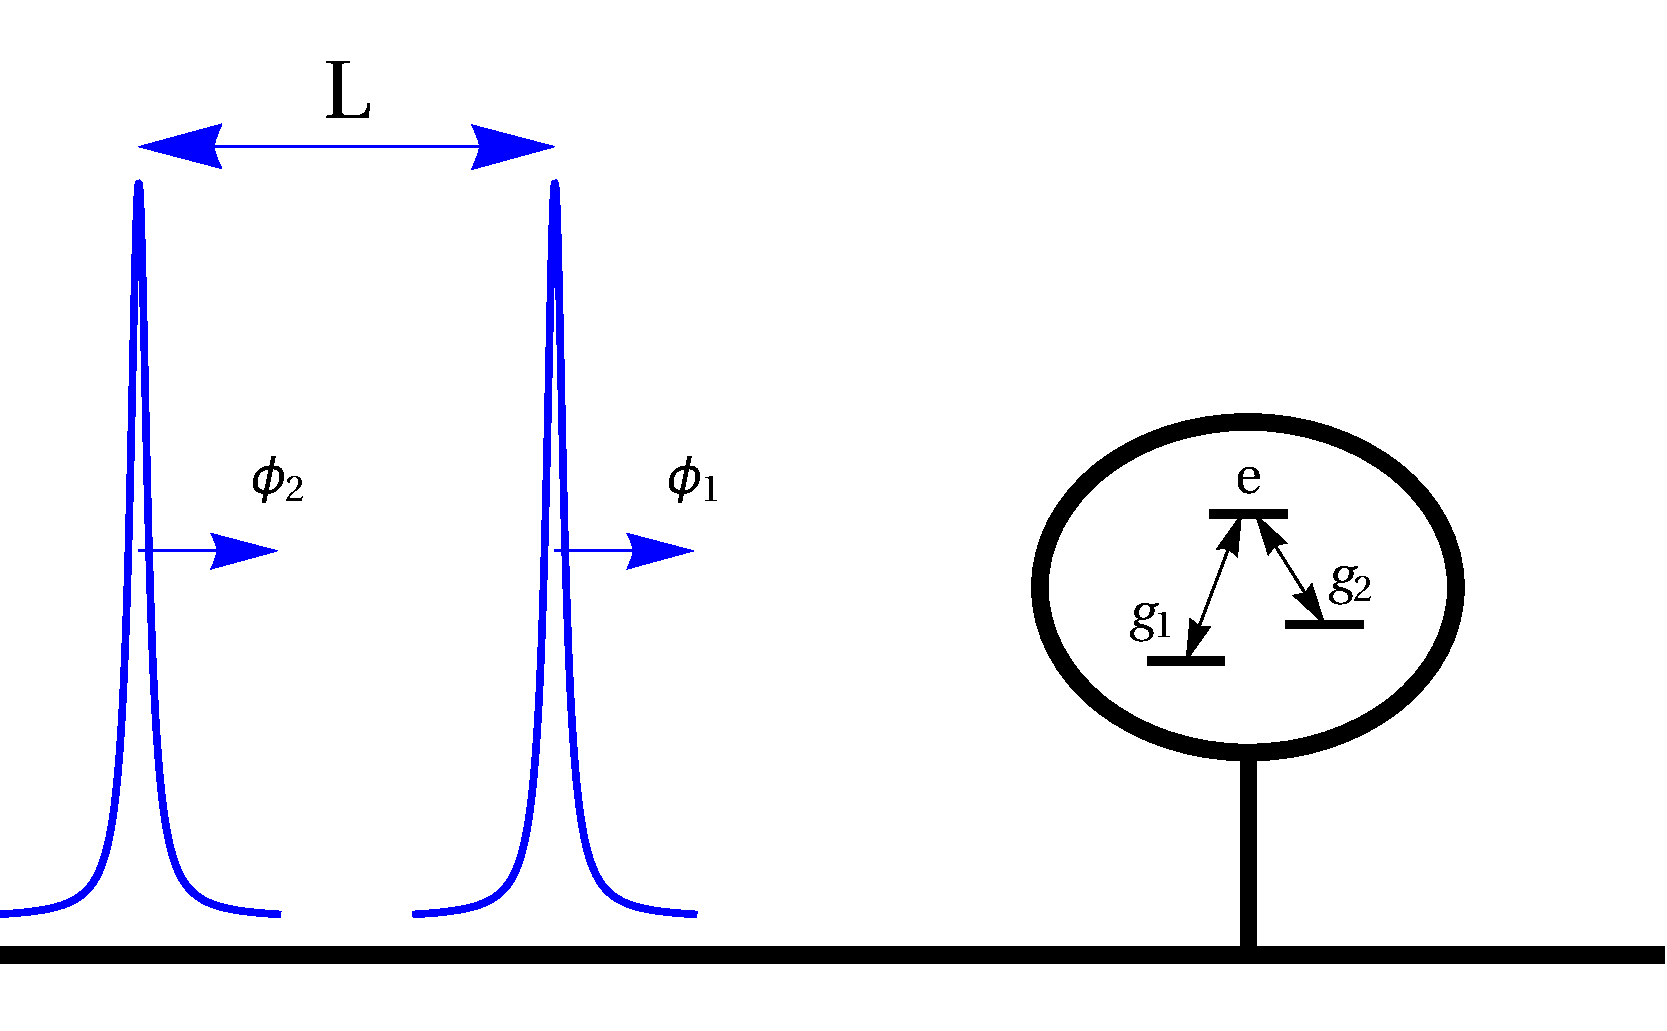
\includegraphics[scale=0.25]{input.pdf}
\caption{Two-photon input state impinging on a $\lambda$ atom. The state $\ket{e}$ is an unstable state which decays to the stable ones, $|g_1\rangle$ and $|g_2\rangle$. The distance $L$ between both wave packets, $\phi_a$ and $\phi_b$, will eventually tend to $\infty$.}
\label{fig:input}
\end{figure}

\section{Free-field causality}

{\color{blue}Bounds for the commutators of the free theory.}

\section{Well-defined scattering}

{\color{blue}Conditions required for having well-defined scattering:

\begin{enumerate}
\item ground state $\simeq$ vacuum far enough from the scatterer,
\item free evolution for the fields far enough from the scatterer, and
\item Fig. with decaying ground state.
\end{enumerate}
}

\section{Cluster revisited}

In this section, we build the ansatz for $S^0$ {\color{blue}(I'm assuming we have already defined $S^0$ and $T$)} in position space. For the sake of simplicity, we first assume we have two photons. The ansatz is
\begin{align}\label{eq:S0_2}
(S^0_{y_1y_2x_1x_2})_{\mu\nu}& = \sum_{\lambda=1}^M \overbrace{(S_{y_1x_1})_{\mu\lambda}(S_{y_2x_2})_{\lambda\nu}}^{\text{single-photon process}}\overbrace{\theta(y_2-y_1)}^\text{causality} \nonumber\\
&+ [x_1\leftrightarrow x_2,y_1\leftrightarrow y_2],
\end{align}
with $x_{1,2}$ the positions of the input photons, $y_{1,2}$ the positions of the output ones, and $|g_\nu\rangle$ and $|g_\mu\rangle$ the initial and final states of the scatterer, respectively. The one-photon matrix $(S_{yx})_{\mu\nu}$ is the amplitude of going from $\ket{x}\otimes \ket{g_\nu}$ to $\ket{y}\otimes \ket{g_\mu}$. Relying on the cluster decomposition principle \cite{weinberg1995}, we take the product of two single-photon $S$ matrices: a photon going from $x_2$ to $y_2$, which induces a transition between  the initial state $|g_\nu\rangle$ and $|g_\lambda\rangle$, $(S_{y_2x_2})_{\lambda\nu}$, and a second photon, which goes from $x_1$ to $y_1$, causing the transition $|g_\lambda\rangle\to |g_\mu\rangle$, $(S_{y_1x_1})_{\mu\lambda}$. Notice there is a summation in the $M$ intermediate stable states of the scatterer, $|g_\lambda\rangle$. We multiply this by a step function ($\theta(y_2-y_1)=1$ if $y_2>y_1$ and $0$ otherwise) to ensure the outgoing photon placed at $y_2$ leaves the scatterer before the photon at $y_1$. Lastly, we symmetrize the result. The generalization for $N$ photons is straightforward
\begin{align}\label{eq:S0_N}
(S^0_{y_1\dots y_N x_1\dots x_N})_{\mu\nu}& = \sum_{\lambda_1\dots \lambda_{N-1}=1}^M\prod_{n=1}^N (S_{y_nx_n})_{\lambda_{n-1}\lambda_n}\nonumber\\
\prod_{m=1}^{N-1}&\theta(y_{m+1}-y_m) + \text{permutations},
\end{align}
with $\lambda_0\equiv \mu$ and $\lambda_N\equiv\nu$. We add all the permutations in $y_n/x_n\leftrightarrow y_m/x_m$ for all $n$ and $m$ in order to symmetrize $S^0$.

Naively, one could build the ansatz \eqref{eq:S0_2} without the step functions. This is valid for scatterers with a unique stable state \cite{Xu2013}. In fact, if we take $M=1$ in Eq. \eqref{eq:S0_2}, we recover this structure without step function
\begin{equation}\label{eq:S0_2_1}
S^0_{y_1y_2x_1x_2} = S_{y_1x_1}S_{y_2x_2} + S_{y_1x_2}S_{y_2x_1}.
\end{equation}
However, the step functions are essential if $M>1$. Otherwise, we would break causality. We consider a two-photon input state
\begin{equation}\label{eq:input}
|\Psi_\text{in}\rangle = \frac{1}{\sqrt{2}}(|\phi_a\rangle \otimes|\phi_b\rangle + |\phi_b\rangle\otimes |\phi_a\rangle)\otimes|g_\nu\rangle,
\end{equation}
where $|\phi_n\rangle$ is a single-photon state. The photon $|\phi_a\rangle$ impinges on the scatterer before $\ket{\phi_b}$ and they are separated by $L\to\infty$, Fig. \ref{fig:input}. Let us compute the probability amplitude of going to the output state
\begin{equation}\label{eq:output}
|\Psi_\text{out}\rangle = \frac{1}{\sqrt{2}}(|\phi_{a'}\rangle \otimes|\phi_{b'}\rangle + |\phi_{b'}\rangle\otimes |\phi_{a'}\rangle)\otimes|g_\mu\rangle,
\end{equation}
which is defined as
\begin{equation}\label{eq:A_def}
A_{ab\to a'b'}^{\nu\to\mu} \equiv \langle \Psi_\text{out}|S|\Psi_\text{in}\rangle.
\end{equation}
We just need the linear part of the $S$ matrix, $S^0$, since both incident wave packets are highly separated. As shown in the Appendix, taking the ansatz given by Eq. \eqref{eq:S0_2}, this probability amplitude is
\begin{equation}\label{eq:A}
A_{ab\to a'b'}^{\nu\to\mu} =  \sum_{\lambda=1}^M A_{a\to a'}^{\nu\to\lambda} A_{b\to b'}^{\lambda\to\mu},
\end{equation}
with $A_{n\to n'}^{\nu\to \mu}\equiv (\langle g_\mu |\otimes \langle \phi_{n'}|)S(|\phi_n\rangle\otimes |g_\nu\rangle)$, that is to say, the probability amplitude for the single-photon process between $|\phi_n\rangle\otimes |g_\nu\rangle$ and $|\phi_{n'}\rangle\otimes |g_\mu\rangle$. Notice this is what one could expect from a standard scattering process: the total amplitude is the product of the amplitudes for both independent events, happening in the proper order. If we did not have included the step function in our ansatz, Eq. \eqref{eq:S0_2}, we would have obtained an unphysical term $A_{b\to b'}^{\nu\to\lambda} A_{a\to a'}^{\lambda\to\mu}$, which says $|\phi_b\rangle$ impinges on the scatterer before $|\phi_a\rangle$, breaking causality.% Details on the computation can be found in the Appendix.

{\color{blue}What about a section with $S^0$ in momentum space?} Taking the Fourier transform of Eq. \eqref{eq:S0_2}, we can compute $S^0$ in momentum space. Before doing so, the single-photon $S$ matrix in momentum space is
\begin{equation}\label{eq:S01_p}
(S_{pk})_{\mu\nu}=t_{\mu\nu}(k)\delta(p+E_\mu-k-E_\nu),
\end{equation}
with $k$ and $p$ the incident and outgoing momenta, respectively, and $|g_\nu\rangle$ and $|g_\mu\rangle$ the initial and final states of the scatterer. The energies $E_\nu$ and $E_\mu$ correspond to the states $|g_\nu\rangle$ and $|g_\mu\rangle$. The factor $t_{\mu\nu}(k)$ is the so-called transmission amplitude. The Dirac delta guarantees energy conservation {\color{blue}WE HAVE TO MENTION SOMEWHERE $v_g=1$}. Then, the two-photon $S^0$ matrix is
\begin{align}\label{eq:S0_2p}
(S_{p_1p_2k_1k_2}^0)_{\mu\nu}=&\frac{1}{(2\pi)^2}\int  dy_1dy_2dx_1dx_2\; (S_{y_1y_2x_1x_2}^0)_{\mu\nu}\nonumber\\
& e^{-i(p_1y_1+p_2y_2)}  e^{i(k_1x_1+k_2x_2)} \nonumber\\
=  \frac{i}{2\pi}\sum_{n,m=1}^2 &\sum_{\lambda=1}^M  \frac{t_{\mu\lambda}(k_n) t_{\lambda\nu}(k_{\overline{n}})}{p_m+E_\mu -k_n -E_\lambda + i0^+}\nonumber\\
&\delta(p_1+p_2+E_\mu - k_1-k_2-E_\nu).
\end{align}
Here, $\overline{n}\neq n$, \emph{e.g.}, $\overline{n}=2$ if $n=1$. The computation is detailed in the Appendix. This structure has recently been found by Xu and Fan in \cite{Xu2016} for a $\lambda$ atom, a three-level atom with two stable states and one unstable state (see the scatterer of Fig. \ref{fig:input}). This is not what one finds in wQED systems if the stable state of the scatterer is unique \cite{Fan2010,Rephaeli2011,Sanchez-Burillo2016b}, as shown in general in \cite{Xu2013}. In that kind of systems, $S^0$ has two Dirac deltas, one for the energy conservation of each photon. We find this structure for $M=1$ (Eqs. \eqref{eq:S0_2_1} and \eqref{eq:S01_p}). In our case, the global Dirac delta imposes energy conservation of the whole process, but each photon does not conserve its energy individually in general. However, for input states like \eqref{eq:input}, they do conserve their energies, as seen in the Appendix, see Eqs. \eqref{eq:energy_conservation} and \eqref{eq:A}. {\color{blue}Say how the photon-photon correlations induced by $S^0$ decay?} %However, for an input state such as \eqref{eq:input}, both photons do conserve its energy individually. The denominator of Eq. \eqref{eq:S0_2p} comes from the Fourier transform of $\theta$ and it is related to the order in which both photons interact with the scatterer.

\section{Connection with input-output theory}\label{sec:inout}

In this section, we set the relation between our ansatz, Eq. \eqref{eq:S0_2}, and the input-output formalism \cite{Gardiner1985}, adapted to wQED problems in \cite{Fan2010}. Concretely, we show what conditions the input-output operators must fulfil so that Eq. \eqref{eq:A} is true.

The input and output states, Eqs. \eqref{eq:input} and \eqref{eq:output}, can be written as a couple of photonic operators acting on the vacuum:
\begin{align}
\label{eq:input_inout}|\Psi_\text{in}\rangle & = \xi_b^\dagger \xi_a^\dagger|\text{vac}\rangle \otimes \ket{g_\nu},\\
\label{eq:output_inout}|\Psi_\text{out}\rangle & = \xi_{b'}^\dagger \xi_{a'}^\dagger|\text{vac}\rangle \otimes \ket{g_\mu},
\end{align}
where $\ket{\text{vac}}$ is the photonic state without particles and $\xi_n^\dagger$ generates a photon whose state is $\ket{\phi_n}$
\begin{equation}
\xi_n^\dagger = \int dx\; \phi_n(x) a_x^\dagger.
\end{equation}
The operator $a_x^\dagger$ creates a photon at $x$. As $\xi_n^\dagger$ is a bosonic operator, both states are already symmetrized. According to the input-output theory, the probability amplitude between both states, Eq. \eqref{eq:A_def}, reads \cite{Fan2010}
\begin{align}\label{eq:A_inout}
A_{ab\to a'b'}^{\nu\to\mu}&=\bra{g_\nu}\otimes\bra{\text{vac}}\xi_{a'}\xi_{b'}\;S\;\xi_b^\dagger\xi_a^\dagger
\ket{\text{vac}}\otimes\ket{g_\nu}\nonumber\\
=\bra{g_\nu}&\otimes\bra{\text{vac}}\xi_{a',\text{out}}\xi_{b',\text{out}}\;\xi_{b,\text{in}}^\dagger\xi_{a,\text{in}}^\dagger
\ket{\text{vac}}\otimes\ket{g_\nu},
\end{align}
where the input and output operators are defined as
\begin{align}
\xi_{n,\text{in}}^\dagger & \equiv e^{iHt_-} e^{-iH_0t_-}\xi_n^\dagger e^{iH_0 t_-} e^{-iHt_-},\\
\xi_{n',\text{out}}^\dagger & \equiv e^{iHt_+} e^{-iH_0t_+}\xi_{n'}^\dagger e^{iH_0 t_+} e^{-iHt_+},
\end{align}
with $t_\pm \to\pm\infty$. {\color{blue}($H$ and $H_0$ should be defined in Section II)}. Provided the following conditions fulfil
\begin{align}
[\xi_{a',\text{out}},\xi_{b,\text{in}}^\dagger]&=0, \label{eq:comm_1} \\
[\xi_{b',\text{out}},\xi_{a,\text{in}}^\dagger]&\neq 0. \label{eq:comm_2}
\end{align}
Eq. \eqref{eq:A_inout} can be rewritten as
\begin{align}
A_{ab\to a'b'}^{\nu\to\mu}=\sum_{\lambda=1}^M&\bra{g_\mu}\otimes\bra{\text{vac}}\xi_{b',\text{out}}\xi_{b,\text{in}}^\dagger \ket{\text{vac}}\otimes\ket{g_\lambda}\nonumber\\
&\bra{g_\lambda} \otimes \bra{\text{vac}} \xi_{a',\text{out}} \xi_{a,\text{in}}^\dagger
\ket{\text{vac}}\otimes\ket{g_\nu},
\end{align}
which is equal to Eq. \eqref{eq:A}, since $A_{n\to n'}^{\nu\to\mu}=\bra{g_\mu}\otimes\bra{\text{vac}}\xi_{n',\text{out}}\xi_{n,\text{in}}^\dagger \ket{\text{vac}}\otimes\ket{g_\nu}$. If Eqs. \eqref{eq:comm_1} and \eqref{eq:comm_2} were false, we would find again noncausal terms, such as $A_{b\to b'}^{\nu\to\lambda}$. In the following, we show that the relations \eqref{eq:comm_1} and \eqref{eq:comm_2} are true.

We can think of the initial state \eqref{eq:input_inout} as if we would have created a photon at a certain time $t$ and a second photon at $t+L$; then, we measure the output, firstly for the first photon and, lastly, for the second one. Thus, commutators \eqref{eq:comm_1} and \eqref{eq:comm_2} can be rewritten in terms of input-output operators in time space \cite{Fan2010}
\begin{align}
\label{eq:comm_a_1}&[a_\text{out}(t),a_\text{in}^\dagger(t+L)]=0,\\
\label{eq:comm_a_2}&[a_\text{out}(t+L),a_\text{in}^\dagger(t)]\neq 0.
\end{align}
We need the equation relating $a_\text{in/out}(t)$ in order to evaluate the previous commutators. For the sake of simplicity, we particularize this computation for a $\lambda$ atom: $M=2$ and an only unstable state, with decay rates $\gamma_1$ and $\gamma_2$. The equation, derived in the Appendix, is
\begin{equation}
\label{eq:a_inout}a_\text{out}(t)=a_\text{in}(t) - i\sqrt{2\gamma_1}\sigma_{1e}(t)-i\sqrt{2\gamma_2}\sigma_{2e}(t),
\end{equation}
with $\sigma_{\lambda e}\equiv \ket{g_\lambda}\bra{e}$. The commutator $[a_\text{out}(t_1),a_\text{in}^\dagger(t_2)]$ is
\begin{align}\label{eq:comm_in_out}
&[a_\text{out}(t_1),a_\text{in}^\dagger(t_2)]=[a_\text{in}(t_1),a_\text{in}^\dagger(t_2)]\nonumber\\
-i&\sqrt{2\gamma_1}[\sigma_{1e}(t_1),a_\text{in}(t_2)]-i\sqrt{2\gamma_2}[\sigma_{2e}(t_1),a_\text{in}(t_2)].
\end{align}
As $a_\text{in/out}(t)$ are bosonic operators \cite{Fan2010} and $t_1\neq t_2$, the first term vanishes. We need the equations of motion of $\sigma_{\lambda e}(t)$ in terms of the input-output operators in order to evaluate the remaining terms. They are also derived in the Appendix. They read
\begin{align}
\label{eq:sigma_inout}\frac{d\sigma_{\lambda e}(t)}{dt}=&-(i\Delta_\lambda+\gamma_1+\gamma_2)\sigma_{\lambda e}(t)\nonumber\\
&+i\left(\sqrt{2\gamma_\lambda}\sigma_{\lambda e}^z(t)-\sqrt{2\gamma_{\overline{\lambda}}}\sigma_{\lambda \overline{\lambda}}(t)\right)a_\text{in}(t),
\end{align}
with $\sigma_{\lambda e}^z\equiv \ket{e}\bra{e}-\ket{g_\lambda}\bra{g_\lambda}$, $\sigma_{\lambda\lambda'}\equiv \ket{g_\lambda}\bra{g_{\lambda'}}$, and $\Delta_\lambda$ the energy gap between $\ket{g_\lambda}$ and $\ket{e}$. In this equation, $\overline{\lambda}\neq \lambda$. Integrating \eqref{eq:sigma_inout} in time from $t_-\to-\infty$ to $t$
\begin{align}
\label{eq:sigma_inout_int}
\sigma_{\lambda e}&(t)-\sigma_{\lambda e}(t_-)=-(i\Delta_\lambda+\gamma_1+\gamma_2)\int_{t_-}^t dt'\sigma_{\lambda e}(t')\nonumber\\
&+i\int_{t_-}^t dt' \left(\sqrt{2\gamma_\lambda}\sigma_{\lambda e}^z(t')- \sqrt{2\gamma_{\overline{\lambda}}}\sigma_{\lambda \overline{\lambda}}(t')\right)a_\text{in}(t').
\end{align}
Taking the commutator between this equation for $t=t_1$ and $a_\text{in}^\dagger(t_2)$
\begin{align}
&[\sigma_{\lambda e}(t_1),a_\text{in}^\dagger(t_2)]=[\sigma_{\lambda e}(t_-),a_\text{in}^\dagger(t_2)]\nonumber\\
&-\left[(i\Delta_\lambda+\gamma_1+\gamma_2)\int_{t_-}^{t_1} dt'\sigma_{\lambda e}(t') \right.\nonumber\\
&\left.+i\int_{t_-}^{t_1} dt' \left(\sqrt{2\gamma_\lambda}\sigma_{\lambda e}^z(t')- \sqrt{2\gamma_{\overline{\lambda}}}\sigma_{\lambda \overline{\lambda}}(t')\right)a_\text{in}(t'),a_\text{in}^\dagger(t_2)\right].
\end{align}
The operator $a_\text{in}^\dagger(t)$ can be written as $a_\text{in}^\dagger(t)=\int dk\; a_k^\dagger (t_-)e^{ik(t-t_-)}/\sqrt{2\pi}$, where $a_k^\dagger$ creates a photon with momentum $k$ \cite{Fan2010}. The commutator $[\sigma_{\lambda e},a_k^\dagger]$ vanishes, since both operators belong to different Hilbert spaces. Then, we conclude the first term of the right hand side is zero. For the other term, as argued in \cite{Xu2015}, the first argument of the commutator just depends on $\{a_\text{in}(t')\}$, for $t_-<t'<t_1$. Thus, if $t_1<t_2$, this commutator is zero, and otherwise it is not. In consequence, $[\sigma_{\lambda e}(t_1),a_\text{in}^\dagger(t_2)]=0$ if $t_1<t_2$ and $[\sigma_{\lambda e}(t_1),a_\text{in}^\dagger(t_2)]\neq 0$ if $t_1>t_2$. Introducing these conditions in \eqref{eq:comm_in_out}
\begin{align}
\label{eq:comm_causality_1}&[a_\text{out}(t_1),a_\text{in}^\dagger(t_2)]=0\quad \text{if}\;\; t_1<t_2,\\
\label{eq:comm_causality_2}&[a_\text{out}(t_1),a_\text{in}^\dagger(t_2)]\neq 0\quad \text{if}\;\; t_1>t_2.
\end{align}
From this, both Eq. \eqref{eq:comm_a_1} and Eq. \eqref{eq:comm_a_2} follow particularizing \eqref{eq:comm_causality_1} for $(t_1,t_2)=(t,t+L)$ and \eqref{eq:comm_causality_2} for $(t_1,t_2)=(t+L,t)$.

We conclude the input-output operators must fulfil the conditions \eqref{eq:comm_causality_1} and \eqref{eq:comm_causality_2} to preserve causality.%Otherwise, the scattering process would not be able to distinguish the order of the incident photons. This condition also applies for systems with a unique stable state. However, in such a case, the probability amplitude \eqref{eq:A} is
%\begin{equation}
%A_{ab\to a'b'}^{1\to 1} =  A_{a\to a'}^{1\to 1} A_{b\to b'}^{1\to 1}.
%\end{equation}
%Thus, the process is not sensitive to the order.

\section{Examples}

{\color{blue}
\begin{enumerate}
\item $\lambda$ atom with 2 photons in momentum space \cite{Xu2016}. Fluorescence from the new part of $S^0$. How the fluorescence decays. MAYBE NOT; IT IS ALREADY EXPLAINED IN SECTION V. I THINK IT MAKES SENSE TO EXPLAIN THIS CASE IN SECTION V BECAUSE IT IS WORTHY TO EXPLAIN THE $S^0$ MATRIX IN MOMENTUM SPACE IN THAT SECTION.
\item Ultrastrong MPS. Fig. with resonance fluorescence. We might include a figure with the decay of the fluorescence as a function of $L$. \cite{Sanchez-Burillo2014,Sanchez-Burillo2015}. Simulations running.
\end{enumerate}
}

\section{Summary and acknowledgements}

In this work...

We have proposed an ansatz for $S^0$ for a point-like scatterer with $M$ stable states, Eqs. \eqref{eq:S0_2} and \eqref{eq:S0_N}. This structure guarantees causality preservation. We have found the conditions the input-output operators must fulfil so that the causality does not break down. In order to show that, the input-output equations for a $\lambda$ atom have been derived.

Summarizing...

We acknowledge...

\appendix

\section{Scattering amplitude}\label{app:A}

We compute the probability amplitude of going from an incident input state to a certain output state in the two-particle subspace. Before, we will need to do the same in the single-photon sector. 

\subsection{One photon}

Let us assume we have an input state with one photon
\begin{equation}
|\Psi_\text{in}^1\rangle=|\phi_a\rangle\otimes |g_\nu\rangle,
\end{equation}
with
\begin{equation}
|\phi_a\rangle\equiv \int dx\; \phi_a(x)|x\rangle.
\end{equation}
The output state will read
\begin{equation}\label{eq:out1}
|\Psi_\text{out}^1\rangle = S|\Psi_\text{in}\rangle = \sum_{\mu=1}^M \int dy dx\;(S_{yx})_{\mu\nu}\phi_a(x)|y\rangle|g_\mu\rangle.
\end{equation}
Defining
\begin{equation}\label{eq:phi_munu}
\phi_{a,\mu\nu}(y)\equiv \int dx\; (S_{yx})_{\mu\nu} \phi_a(x)
\end{equation}
and
\begin{equation}\label{eq:out_munu}
|\psi_\text{out}^1\rangle_{a,\mu\nu}\equiv \int dy\;\phi_{a,\mu\nu}(y) |y\rangle
\end{equation}
the output state \eqref{eq:out1} can be rewritten as
\begin{equation}
|\Psi_\text{out}^1\rangle = \sum_{\mu=1}^M |\psi_\text{out}^1\rangle_{a,\mu\nu}\otimes |g_\mu\rangle.
\end{equation}
The probability amplitude $A_{a\to a'}^{\nu\to\mu}$ will be
\begin{equation}\label{eq:A1}
A_{a\to a'}^{\nu\to\mu} = \langle g_\mu|\otimes \langle \phi_{a'}|S|\phi_a\rangle \otimes |g_\nu\rangle = \langle \phi_{a'}|\psi_\text{out}\rangle_{a,\mu\nu}.
\end{equation}
Provided both $|\phi_a\rangle$ and $|\phi_{a'}\rangle$ are monochromatic states with momenta $k$ and $p$, respectively, this amplitude is
\begin{equation}\label{eq:energy_conservation}
A_{a\to a'}^{\nu\to\mu} = \sum_{\mu=1}^M (S_{pk})_{\mu\nu}.
\end{equation}

\subsection{Two photons}

We now assume we have a two-photon input state like that shown in Fig. \ref{fig:input}
\begin{equation}\label{eq:input2}
|\Psi_\text{in}^2\rangle = \frac{1}{\sqrt{2}}(|\phi_a\rangle\otimes|\phi_b\rangle+|\phi_b\rangle\otimes|\phi_a\rangle)\otimes|g_\nu\rangle.
\end{equation}
By definition, the output state is
\begin{equation}
|\Psi_\text{out}^2\rangle = S^0|\Psi_\text{in}^2\rangle.
\end{equation}
We just take into account the linear part of the scattering matrix because the incident photons are far away. We introduce the identity operator
\begin{equation}\label{eq:out2}
|\Psi_\text{out}^2\rangle = \mathbb{I}S^0\mathbb{I}|\Psi_\text{in}^2\rangle,
\end{equation}
with
\begin{equation}\label{eq:I}
\mathbb{I}=\frac{1}{2}\sum_{\mu=1}^M \int dx_1dx_2\;|x_1x_2;g_\nu\rangle \langle x_1x_2;g_\nu|,
\end{equation}
being $|x_1x_2;g_\nu\rangle$ the symmetrized state
\begin{equation}
|x_1x_2;g_\nu\rangle=\frac{1}{\sqrt{2}}(|x_1\rangle\otimes|x_2\rangle + |x_2\rangle\otimes|x_1\rangle)\otimes \ket{g_\nu}.
\end{equation}
Introducing \eqref{eq:I} in \eqref{eq:out2} and considering \eqref{eq:input2} and \eqref{eq:S0_2}
\begin{align}\label{eq:out2_2}
|\Psi_\text{out}^2\rangle = &\frac{1}{4}\int dy_1dy_2dx_1dx_2\nonumber\\
&\sum_{\mu,\lambda=1}^M\sum_{n,m=1}^2(S_{y_nx_m})_{\mu\lambda} (S_{y_{\overline{n}}x_{\overline{m}}})_{\lambda\nu}\theta(y_{\overline{n}}-y_n)\nonumber\\
&(\phi_a(x_1)\phi_b(x_2)+\phi_a(x_2)\phi_b(x_1))|y_1y_2;g_\mu\rangle.
\end{align}
We have to compute integrals such as
\begin{align}
C=\int dx_1dx_2\;\sum_{n,m}&(S_{y_nx_m})_{\mu\lambda} (S_{y_{\overline{n}}x_{\overline{m}}})_{\lambda\nu}\nonumber\\
&\phi_i(x_1)\phi_j(x_2)\theta(y_{\overline{n}}-y_n).
\end{align}
Using Eq. \eqref{eq:phi_munu}
\begin{align}\label{eq:C1}
C=\sum_{n=1}^2(&\phi_{i,\mu\lambda}(y_n)\phi_{j,\lambda\nu}(y_{\overline{n}}) \nonumber\\
& + \phi_{j,\mu\lambda}(y_n)\phi_{i,\lambda\nu}(y_{\overline{n}}))\theta(y_{\overline{n}}-y_n).
\end{align}
The functions $\phi_a(x)$ and $\phi_b(x)$ are such that, if $\phi_a(x_m)\phi_b(x_{\overline{m}})$ is different from zero, then $x_m>x_{\overline{m}}$, Fig. \ref{fig:input}. The same applies for $\phi_{a,\mu\nu}(y_n)\phi_{b,\mu\nu}(y_{\overline{n}})$. Notice that the previous expression is different from zero just if $y_{\overline{n}}>y_n$, since we have the step function. If $i=a$ and $j=b$, the first term is zero and the step function is irrelevant, so $C$ will read
\begin{align}\label{eq:C2}
C=\sum_{n=1}^2\phi_{b,\mu\lambda}(y_n)\phi_{a,\lambda\nu}(y_{\overline{n}})).
\end{align}
One can easily see that the same expression is true if $i=b$ and $j=a$. Then, the output state, Eq. \eqref{eq:out2_2} is
\begin{align}
|\Psi_\text{out}^2\rangle &=\frac{1}{2\sqrt{2}}\int dy_1dy_2\;\sum_{\mu,\lambda=1}^M(\phi_{b,\mu\lambda}(y_1)\phi_{a,\lambda\nu}(y_2)\nonumber\\
+&\phi_{b,\mu\lambda}(y_2)\phi_{a,\lambda\nu}(y_1))(|y_1\rangle\otimes|y_2\rangle + |y_2\rangle\otimes|y_1\rangle)\otimes|g_\mu\rangle.
\end{align}
Introducing Eq. \eqref{eq:out_munu}
\begin{align}\label{eq:out_final}
|\Psi_\text{out}^2\rangle =&\frac{1}{\sqrt{2}}\sum_{\mu,\lambda=1}^M(|\psi_\text{out}^1\rangle_{b,\mu\nu}\otimes|\psi_\text{out}^1\rangle_{a,\nu\lambda}  \nonumber\\
& + |\psi_\text{out}^1\rangle_{a,\nu\lambda}\otimes|\psi_\text{out}^1\rangle_{b,\mu\nu})\otimes|g_\mu\rangle.
\end{align}
Finally, the probability amplitude of going to the output state
\begin{equation}
\frac{1}{\sqrt{2}}(|\phi_{a'}\rangle\otimes|\phi_{b'}\rangle+|\phi_{b'}\rangle\otimes|\phi_{a'}\rangle)\otimes|g_\mu\rangle
\end{equation}
will be the overlap between this state and \eqref{eq:out_final}. Using \eqref{eq:A1}
\begin{equation}
A_{ab\to a'b'}^{\nu\to\mu}=\sum_{\lambda=1}^M A_{a\to a'}^{\nu\to\lambda} A_{b\to b'}^{\lambda\to\mu},
\end{equation}
as expected, where we have chosen $|\phi_{m'}\rangle$ such that $A_{n\to m'}^{\nu\to \mu}=0$ if $n\neq m$. If we would not have considered the step functions, we would have obtained the unphysical amplitude $A_{b\to b'}^{\nu\to\lambda} A_{a\to a'}^{\lambda\to\mu}$ when going from \eqref{eq:C1} to \eqref{eq:C2}.


\section{$S^0$ in momentum space}\label{app:Sp}

We show $S^0$ in momentum space follows Eq. \eqref{eq:S0_2p}. For the sake of simplicity, we focus on $N=2$ so we start from Eq. \eqref{eq:S0_2}. By definition, $(S^0_{p_1p_2k_1k_2})_{\mu\nu}$ reads
\begin{align}\label{eq:App_1}
(S_{p_1p_2k_1k_2}^0)_{\mu\nu}=&\frac{1}{(2\pi)^2}\int  dy_1dy_2dx_1dx_2\; (S_{y_1y_2x_1x_2}^0)_{\mu\nu}\nonumber\\
& e^{-i(p_1y_1+p_2y_2)}  e^{i(k_1x_1+k_2x_2)},
\end{align}
with $(S_{y_1y_2x_1x_2}^0)_{\mu\nu}$ given by \eqref{eq:S0_2}. We will have integrals such as
\begin{equation}
I=\int dx\; e^{ikx}(S_{yx})_{\mu\nu}.
\end{equation}
As $(S_{yx})_{\mu\nu}$ is just the Fourier transform of $(S_{pk})_{\mu\nu}$ (Eq. \eqref{eq:S01_p}), the former integral will be
\begin{equation}
I=e^{i(k+E_\nu-E_\mu)y}t_{\mu\nu}(k).
\end{equation}
Introducing this in \eqref{eq:App_1}
\begin{align}\label{eq:App_2}
(S_{p_1p_2k_1k_2}^0)_{\mu\nu}=\frac{1}{(2\pi)^2} &\int dy_1 dy_2\; e^{-i(p_1y_1+p_2y_2)}\nonumber\\
\sum_{n,m=1}^2 \sum_{\lambda=1}^M e^{i(k_ny_1 + k_{\overline{n}} y_2)}& e^{i[(E_\lambda-E_\mu)y_m+(E_\nu-E_\lambda)y_{\overline{n}}]} \nonumber\\
t_{\mu\lambda}(k_n)t_{\lambda\nu}(k_{\overline{n}})& \theta(y_{\overline{m}}-y_m),
\end{align}
with $\overline{n}(\overline{m})\neq n(m)$. The Fourier transform of the step function is
\begin{equation}
\frac{1}{\sqrt{2\pi}}\int dy \; e^{-iqy}\theta(\mp(y-y_0))=\pm\frac{i}{\sqrt{2\pi}}\frac{e^{-iqy_0}}{q\pm i0^+}.
\end{equation}
Integrating Eq. \eqref{eq:App_2} in $y_1$
\begin{align}
(S_{p_1p_2k_1k_2}^0)_{\mu\nu}=&\frac{i}{(2\pi)^2} \int dy_2\; e^{-i(p_1+p_2+E_\mu-k_1-k_2-E_\nu)y_2} \nonumber\\
\sum_{n=1}^2 & \left( \frac{t_{\mu\lambda}(k_n)t_{\lambda\nu}(k_{\overline{n}})}{p_1+E_\mu-k_n-E_\lambda+i0^+} \right. \nonumber\\
&\left. -\frac{t_{\mu\lambda}(k_n)t_{\lambda\nu}(k_{\overline{n}})}{p_1+E_\lambda-k_n-E_\nu-i0^+}\right).
\end{align}
Notice the integral in $y_2$ gives a Dirac delta. Thus
\begin{align}
(S_{p_1p_2k_1k_2}^0)_{\mu\nu}=&\frac{i}{2\pi} \delta(p_1+p_2+E_\mu-k_1-k_2-E_\nu) \nonumber\\
\sum_{n=1}^2 \sum_{\lambda=1}^M& \left( \frac{t_{\mu\lambda}(k_n)t_{\lambda\nu}(k_{\overline{n}})}{p_1+E_\mu-k_n-E_\lambda+i0^+} \right. \nonumber\\
&\left. -\frac{t_{\mu\lambda}(k_n)t_{\lambda\nu}(k_{\overline{n}})}{p_1+E_\lambda-k_n-E_\nu-i0^+}\right).
\end{align}
Applying the condition imposed by the Dirac delta to the denominator of the third row
\begin{align}
(S_{p_1p_2k_1k_2}^0)_{\mu\nu}=  &\frac{i}{2\pi}\sum_{n,m=1}^2 \sum_{\lambda=1}^M  \frac{t_{\mu\lambda}(k_n) t_{\lambda\nu}(k_{\overline{n}})}{p_m+E_\mu -k_n -E_\lambda + i0^+}\nonumber\\
&\delta(p_1+p_2+E_\mu - k_1-k_2-E_\nu),
\end{align}
which is the expression given in the main text, Eq. \eqref{eq:S0_2p}. This result has been recently reported for a $\lambda$ atom and different local scatterers by Xu and Fan \cite{Xu2016}. Here, we show this is completely general, according to our ansatz (Eq. \eqref{eq:S0_2}).

%\begin{figure}[tbh!]
%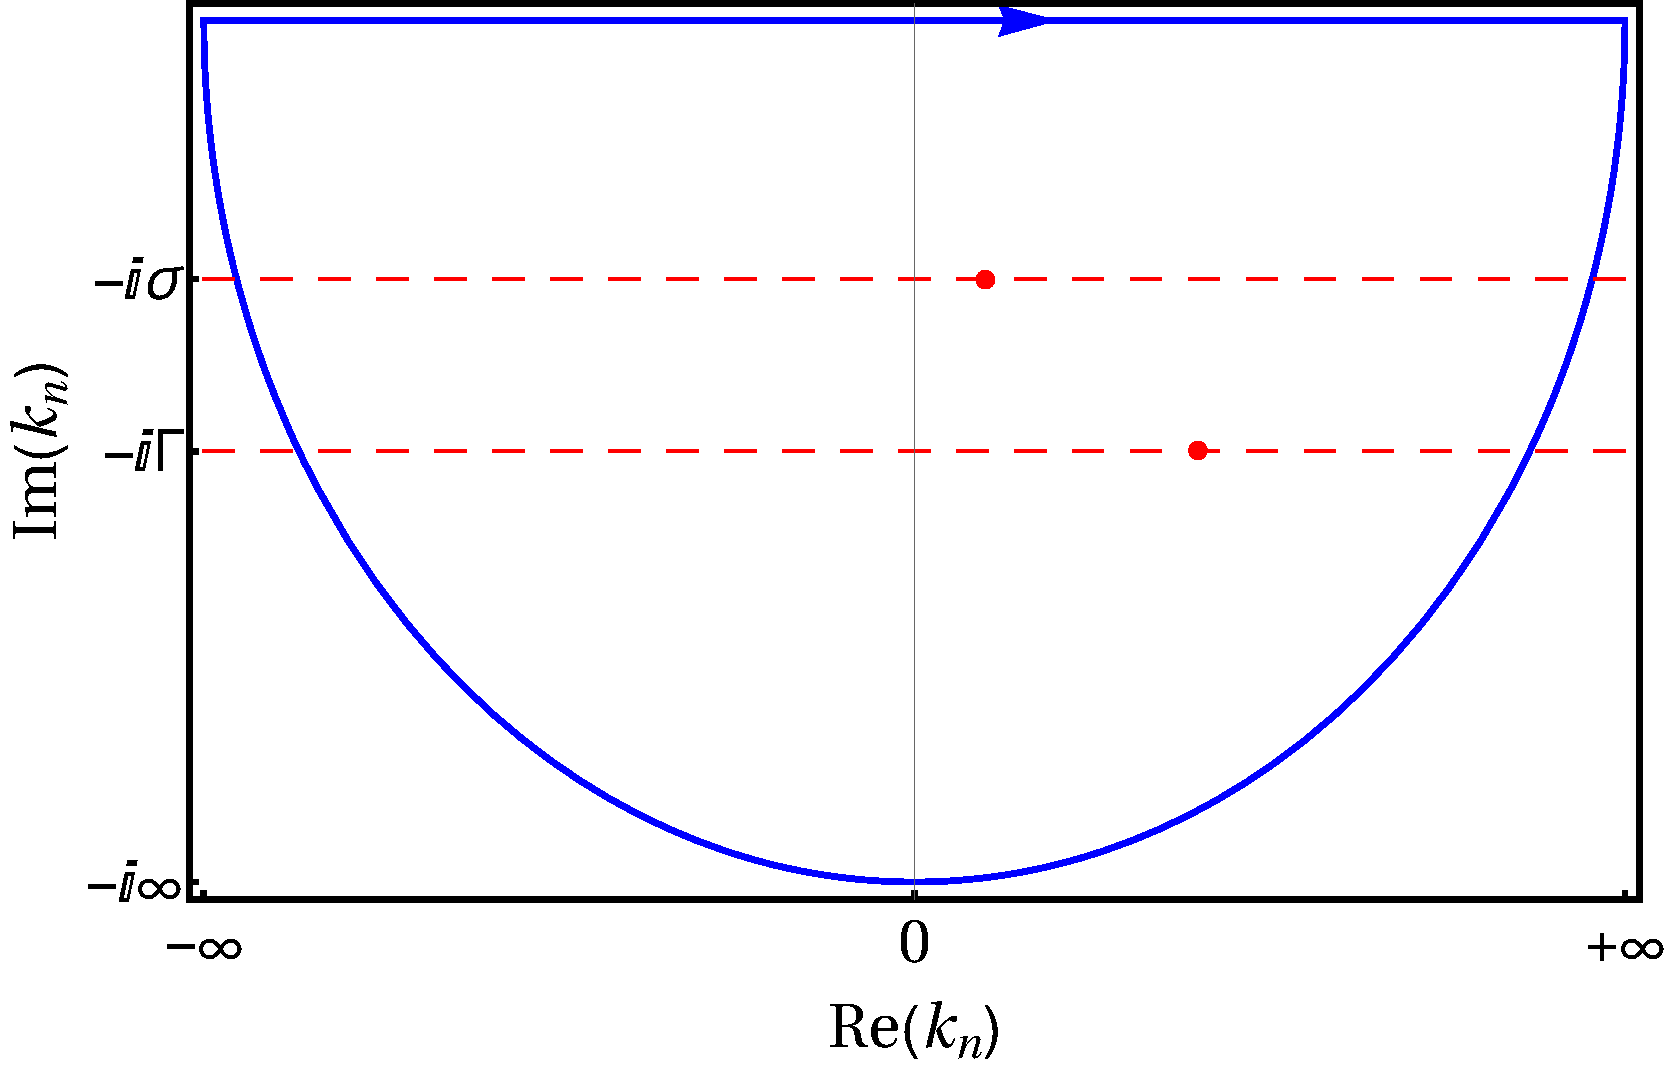
\includegraphics[scale=0.25]{lower_contour.pdf}
%\caption{Integration contour for Eq. (...). The red points are the poles of the
%integrand. The values of the real parts are arbitrary.}
%\label{fig:lower}
%\end{figure}

%\begin{figure}[tbh!]
%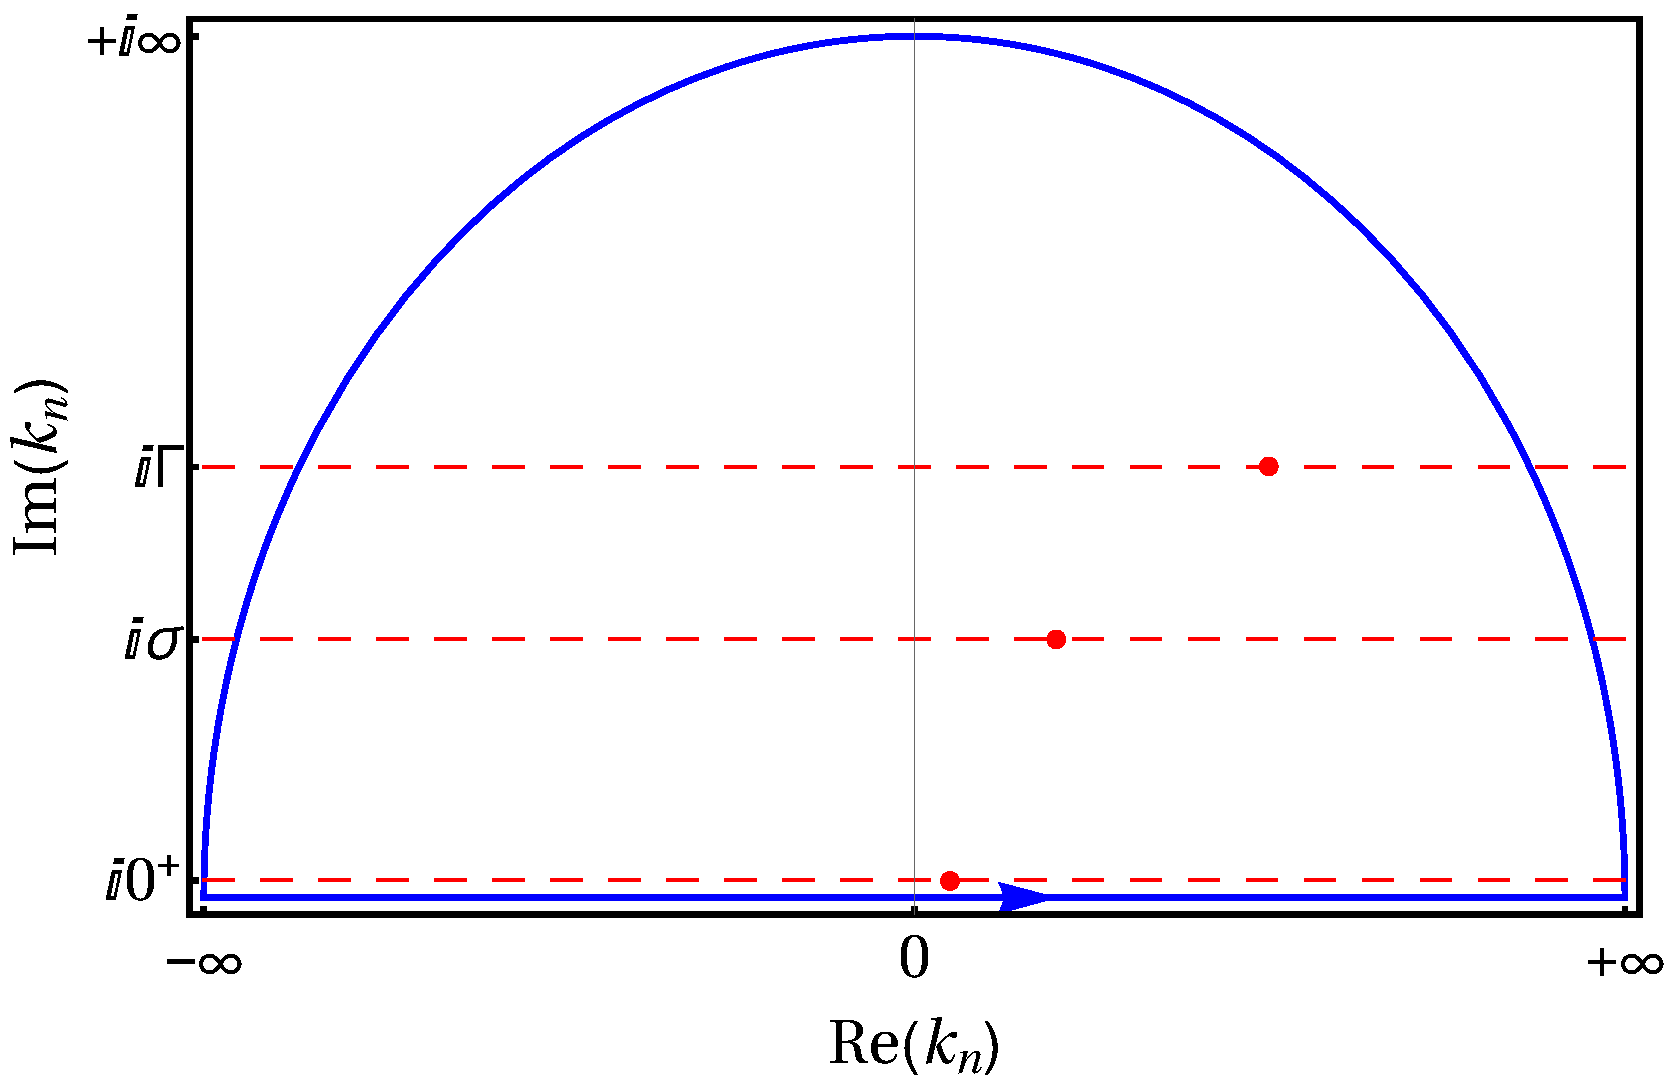
\includegraphics[scale=0.25]{upper_contour.pdf}
%\caption{Integration contour for Eq. (...). The red points are the poles of the
%integrand. The values of the real parts are arbitrary.}
%\label{fig:upper}
%\end{figure}

\section{Input-output equations for a $\lambda$ atom}

In this section of the Appendix we derive the input-output equations \eqref{eq:a_inout} and \eqref{eq:sigma_inout}. We start from the Hamiltonian for a chiral one-dimensional waveguide coupled to a $\lambda$ atom
\begin{align}
H & = \int d\omega \; \omega a_\omega^\dagger a_\omega + E_1\ket{1}\bra{1} + E_2\ket{2}\bra{2} + E_e\ket{e}\bra{e}\nonumber\\
& + \int d\omega\; (g_1\sigma_{1e}^\dagger a_\omega + g_2 \sigma_{2e}^\dagger a_\omega + \text{H.c.}).
\end{align}
%Subtracting $E_1$
%\begin{align}
%H & = \int d\omega \; \omega a_\omega^\dagger a_\omega + \Delta_1\sigma_{1e}^\dagger\sigma_{1e} + \Delta_2 \sigma_{2e}^\dagger\sigma_{2e} \nonumber\\
%& + \int d\omega\; (g_1\sigma_{1e}a_\omega + g_2 \sigma_{2e} a_\omega + \text{H.c.}),
%\end{align}
%with $\Delta_\lambda\equiv E_e-E_\lambda$. The operators $\sigma_{\lambda e}=\ket{g_\lambda}\bra{e}$ were defined in the main text (Section \ref{sec:inout}).
We need to know the Heisenberg equations, $d\mathcal{O}/dt=i[H,\mathcal{O}]$, in order to derive the input-output ones. The Heisenberg equation for $a_\omega(t)$ is
\begin{equation}\label{eq:aw_Heisenberg}
i\frac{d a_\omega(t)}{dt}=\omega a_\omega(t) + g_1 \sigma_{1e}(t) + g_2 \sigma_{2e}(t).
\end{equation}
For $\sigma_{\lambda e}(t)$
\begin{align}\label{eq:sigma_Heisenberg}
&i\frac{d\sigma_{\lambda e}(t)}{dt}=\Delta_\lambda \sigma_{\lambda e}(t)\nonumber\\
&-\int d\omega\; (g_\lambda \sigma_{\lambda e}^z(t)-g_{\overline{\lambda}} \sigma_{\lambda\overline{\lambda}}(t))a_\omega(t),
\end{align}
where the gap $\Delta_\lambda=E_e-E_\lambda$ and the operators $\sigma_{\lambda e}^z=\ket{e}\bra{e}-\ket{g_\lambda}\bra{g_\lambda}$ and $\sigma_{\lambda\overline{\lambda}}=\ket{g_\lambda}\bra{g_{\overline{\lambda}}}$ have already been defined in the main text. As before, $\overline{\lambda}\neq \lambda$.

Evaluationg Eq. \eqref{eq:aw_Heisenberg} at $t=t'$, multiplying it by $e^{i\omega t'}$ and integrating $t'$ from $t_-\to -\infty$ to $t$
\begin{align}\label{eq:aw_t}
&a_\omega(t)=e^{-i\omega(t-t_-)} a_\omega(t_-)\nonumber\\
& - i\sum_{\lambda=1}^2 g_\lambda \int_{t_-}^t dt'\; \sigma_{\lambda e}(t')e^{-i\omega(t-t')}.
\end{align}
I define
\begin{align}
\label{eq:Phi}\Phi(t) & \equiv \frac{1}{\sqrt{2}}\int d\omega\; a_\omega (t),\\
a_\text{in}(t) & \equiv \frac{1}{\sqrt{2}}\int d\omega\; a_\omega(t_-) e^{-i\omega(t-t_-)},\\
a_\text{out}(t) & \equiv \frac{1}{\sqrt{2}}\int d\omega\; a_\omega(t_+) e^{-i\omega(t-t_+)},
\end{align}
with $t_\pm\to \pm\infty$. Integrating Eq. \eqref{eq:aw_t} with respect to $\omega$ and taking into account that the decay rates are related to the coupling constants as $\gamma_\lambda=\pi g_\lambda^2$
\begin{equation}\label{eq:phi_in}
\Phi(t)=a_\text{in}(t)-i\sum_{\lambda=1}^2\sqrt{\frac{\gamma_\lambda}{2}} \sigma_{\lambda e}(t).
\end{equation}
Evaluationg Eq. \eqref{eq:aw_Heisenberg} at $t=t'$, multiplying it by $e^{i\omega t'}$ and integrating $t'$ from $t$ to $t_+\to +\infty$
\begin{equation}\label{eq:phi_out}
\Phi(t)=a_\text{out}(t)+i\sum_{\lambda=1}^2\sqrt{\frac{\gamma_\lambda}{2}} \sigma_{\lambda e}(t).
\end{equation}
From Eqs. \eqref{eq:phi_in} and \eqref{eq:phi_out}
\begin{equation}
a_\text{out}(t)=a_\text{in}(t)-i\sum_{\lambda=1}^2 \sqrt{2\gamma_\lambda} \sigma_{\lambda e}(t),
\end{equation}
which is equal to Eq. \eqref{eq:a_inout}. Introducing \eqref{eq:phi_in} in \eqref{eq:sigma_Heisenberg}, taking into account the definition of $\Phi(t)$ \eqref{eq:Phi}
\begin{align}
\frac{d\sigma_{\lambda e}(t)}{dt}=&-(i\Delta_\lambda +\gamma_1+\gamma_2)\sigma_{\lambda e}(t)\nonumber\\
&+i(\sqrt{2\gamma_\lambda} \sigma_{\lambda e}^z(t) - \sqrt{2\gamma_{\overline{\lambda}}}\sigma_{\lambda\overline{\lambda}}(t))a_\text{in}(t),
\end{align} 
which is equal to \eqref{eq:sigma_inout}.

\section{Matrix Product States}

As we indicated in the main text, we solve the ultrastrong example by means of the MPS technique. We explain the method and justify why we can use it, as we already did in \cite{Sanchez-Burillo2014,Sanchez-Burillo2015,Sanchez-Burillo2016a}.

Our photonic medium can be treated in the RWA and its ground state is the vacuum both in frequency and position space. Moreover, even if we go beyond RWA in the scatterer-resonator coupling ($g/\Delta\gtrsim 0.1$), it is true that the ground state is not the vacuum anymore, as we showed in \cite{Sanchez-Burillo2014}, but it will follow the area law \cite{Eisert2010}, so it will be slightly entangled. As we are studying the dynamics of two photons flying over the ground state, the state will have a small amount of entanglement.

The main consequence of the previous discussion is that we may use the variational ansatz of Matrix Product States \cite{Ripoll2006,Verstraete2008} to describe the discrete wavefunction, since it is valid for 1D systems when the entanglement is small enough. This ansatz has the form
\begin{equation}
\ket{\psi} = \sum_{s_i \in \{1,d_i\}} \mathrm{tr}\left[
\prod A_i^{s_i}\right] \ket{s_1,s_2,\ldots,s_L}.
\label{eq:mps}
\end{equation}
It is constructed from $L$ sets of complex matrices $A_i^{s_i} \in M[\mathbb{C}^{D}]$, where each set is labeled by the quantum state $s_i$ of the corresponding site. The local Hilbert space dimention $d_i$ is infinity, since we are dealing with bosonic sites. However, during the dynamics, processes creating multiple photons are still highly off-resonance. Thus, we can truncate the bosonic space and consider states with $0$ to
$n_\text{max}$ photons per cavity. So, the composite Hilbert space is $\mathcal{H}=\bigotimes_i \mathbb{C}^{d_i}$, where the dimension is $d_i=n_\text{max}+1$ for the empty resonators and $d_{i_0}=n_\text{scatt}(n_\text{max}+1)$ for the cavity with the scatterer, where $n_\text{scatt}$ is the number of levels of the scatterer. We thus expect the composite wavefunction of the photon-scatterer system to consist of a superposition with a small number of photons

The total number of variational parameters $(L-1)D^2(n_\text{max}+1) + n_\text{scatt}D^2(n_\text{max}+1)$, depends on the size of the matrices, $D$. The key point is that, for describing a general state, $D$ increases exponentially with $L$, whereas its dependence is polynomial if the entanglement is small enough, in such a way that the number of parameters increases polynomially with $L$ for this class of states.

Our work with MPS relies on four different algorithms. The most basic one is to create trivial, product states of known shape, such as a vacuum state with the scatterer in the ground state $\ket{\psi}=\ket{\text{vac}}\otimes \ket{g_1}$. These states can be reproduced using matrices of bond dimension $D=1$, so each matrix is just a coefficient $A_i^{s_i}=\delta_{s_i1}$. The second algorithm is to compute expectation values from MPS. This amounts to a contraction of tensors that can be performed efficiently \cite{Ripoll2006}, and allows us to compute single-site operators $\langle a^\dagger_i a_i\rangle$, $\langle \sigma_z\rangle$, or correlators, $\langle a_i^\dagger a_j\rangle$. The third operation that we need to perform is to apply operators on to the state, $\mathcal{O}\ket{\psi}$, such as introducing or removing excitations $a_i^\dagger\ket{\psi}$. We do this in an efficient fashion by interpreting the operator $\mathcal{O}$ as a Matrix Product Operator (MPO) \cite{Pirvu2010}. A MPO is a matrix product representation of an operator:

\begin{equation}
\mathcal{O} = \sum_{s_{i}^{},s_{i}^\prime \in \{1,d_i\}} \mathrm{tr}\left[\prod B_i^{s_i^{},s_i^\prime}\right]\ket{s_1^{},s_2^{},\ldots,s_L^{}}\bra{s_1^\prime,s_2^\prime,\ldots,s_L^\prime}
\end{equation}

So, now we have $L$ sets of complex matrices $B_i^{s_i^{},s_i^\prime} \in M[\mathbb{C}^{D_\mathcal{O}}]$, where each set is labeled by two indices $s_i^{},s_i^\prime$ of the corresponding site.

We just need to apply sums of one-body operators

\begin{equation}
\mathcal{O} = a_\phi^\dagger = \sum_n \phi_n a_n^\dagger.
\end{equation}

In such a case, an efficient representation of the MPO is obtained with $D_\mathcal{O}=2$

\begin{equation}
B_i^{s_i^{},s_i^\prime}=\left(\begin{array}{c c}
\delta_{s_i^{},s_i^\prime} & 0\\
\phi_i(a_i^\dagger)_{s_i^{},s_i^\prime} & \delta_{s_i^{},s_i^\prime}
\end{array}\right)\qquad i=2,3,\dots,L-1,
\end{equation}
whereas $B_1^{s_1^{},s_1^\prime}=(\phi_1(a_1^\dagger)_{s_1^{},s_1^\prime},\delta_{s_1^{},s_1^\prime})$ and $B_L^{s_L^{},s_L^\prime}=(\delta_{s_L^{},s_L^\prime},\phi_L(a_L^\dagger)_{s_L^{},s_L^\prime})^T$, with $(a_i^\dagger)_{s_i^{},s_i^\prime}=:\bra{s_i^{}}a_i^\dagger\ket{s_i^\prime}$.

Finally, with this tool in our box, we can also approximate time evolution, repeatedly contracting the state with an MPO approximation of the unitary operator $\exp(-iH\Delta t)$ for short times, and truncating it to an ansatz with a fixed $D$. Since our problem does not contain long-range interactions and since the state is well approximated by MPS, it is sufficient to rely on a third-order Suzuki-Trotter formula \cite{Suzuki1991}.
In the same way as we can consider time evolution, we can take imaginary time to obtain the ground state and excited states, that is solving the equation $i\tfrac{d}{dt}P\ket{\psi}=PHP\ket{\psi}$ for finite time-steps, while constantly renormalizing the state. Here, $P$ is either the identity (for the ground state) or a projector that either selects a well defined quantum number (parity $\Pi$) or projects out already computed states. In either case, provided a suitable initial state, the algorithm converges to the lowest-energy state of $H$ in the subspace selected by $P$.

\bibliographystyle{apsrev4-1}
\bibliography{bib_cluster}



\end{document}